\documentclass{article}

\usepackage{geometry}
\usepackage[hidelinks, bookmarks = true]{hyperref}
\usepackage[numbered]{bookmark}
\usepackage{booktabs}
\usepackage{float}
\usepackage{graphicx}
\usepackage{geometry}
\usepackage{titletoc}
\usepackage{indentfirst}
\usepackage{fancyhdr} 
\usepackage{longtable}
\usepackage{supertabular}
\usepackage[normalem]{ulem}
\usepackage{listings}
\usepackage{xcolor}
\usepackage{xurl}
\usepackage{tikz}
\usepackage{lastpage}
\usepackage{amsmath}
\usepackage{amssymb}
\usepackage{mathtools}
\usepackage{caption}
\usepackage{threeparttable}
\usepackage{subcaption}

\geometry{a4paper, left = 1.9cm, right = 1.9cm, top = 2.3cm, bottom = 2.3cm, includehead}
\captionsetup[table]{font={small}}

\pagestyle{fancy}
\fancyhead[R]{\thepage /\pageref{LastPage}}
\fancyhead[L]{GROUP 28}
\fancyfoot{}
\fancyfoot{}
\renewcommand{\headrulewidth}{0pt}
\renewcommand{\footrulewidth}{0pt}
\setlength{\headheight}{14.49998pt}
\addtolength{\topmargin}{-2.49998pt}

\begin{document}
\noindent\rule{\textwidth}{1pt}
\begin{center}
    \LARGE \textbf{Assignment 2: Predict Future Sales}
\end{center}
\noindent\rule{\textwidth}{0.5pt}
\begin{center}
    \textbf{Group 28}\par
    \vspace{0.3cm}
Shuang Fan\phantom{space}Kaiteng Jiang\phantom{space}Shupei Li\\
s3505847\phantom{spacespac}s3479420\phantom{spacespa}s3430863
\end{center}
    \vspace{0.2cm}
\textbf{Kaggle team name: AiDM-Group 28}

\section{Problem Statement}
This Kaggle competition is related to tabular data and time-series algorithms. Datasets are provided by a Russian software company. The training set is the daily sales data from January 2013 to October 2015. The target of the competition is predicting the sales in November 2015 for each shop-item pair. Except for historical sales data, other useful information includes meta data of item, category, and shop.

\section{Exploratory Data Analysis}
We explore datasets via descriptive statistics and data visualization. The following is our findings.

\subsection{Descriptive Statistics}\label{stat}
First, we count the number of shops and items in the datasets. There are 60 shops and 21,807 items in the train set, 40 shops and 5,100 items in the test set. However, the test set includes 363 items that are not in the train set. It is worth noting that there is no missing value in datasets. Then, we calculate primary descriptive statistics of the training set to provide an overview of the data. Table \ref{tab:de-stat} reports the results.

\begin{table}[!ht]
    \centering
    \caption{Summary of Descriptive Statistics}
    \label{tab:de-stat}
    \begin{threeparttable}
    \begin{tabular}{llllllll}
        \toprule
        \textbf{Variable} & \textbf{Mean} & \textbf{Std.} & \textbf{Min} & \textbf{Median} & \textbf{Max} & \textbf{\#Negative Records}\\
        \midrule
        Item Price & 890.9 & 1,729.8 & -1 & 399 & 307,980 & 1\\
        Daily Sales & 1.2 & 2.6 & -2.2 & 1 & 2,169 & 7,356\\
        Total Sales by Category* & 43,431.0 & 99,846.0 & 1 & 9,515.5 & 634,171 & -\\
        \bottomrule
    \end{tabular}
    \begin{tablenotes}
        \footnotesize
        \item[*] The number of categories is 84.
    \end{tablenotes}
    \end{threeparttable}
\end{table}

According to Table \ref{tab:de-stat}, there are anomalies in item price and daily sales, i.e., negative values. We deal with these anomalies at the stage of preprocessing. Besides, we notice that the maximum of item price may be too high. We further investigate possible outliers in the item price by drawing box lpots. Figure \ref{fig:price-box} shows the box plots with and without outliers. The outlier of item price is significant, with a maximum value over 300,000 that deviates from the normal range. We need to take over highly prices into consideration when creating features. 

\begin{figure}[!ht]
    \centering
    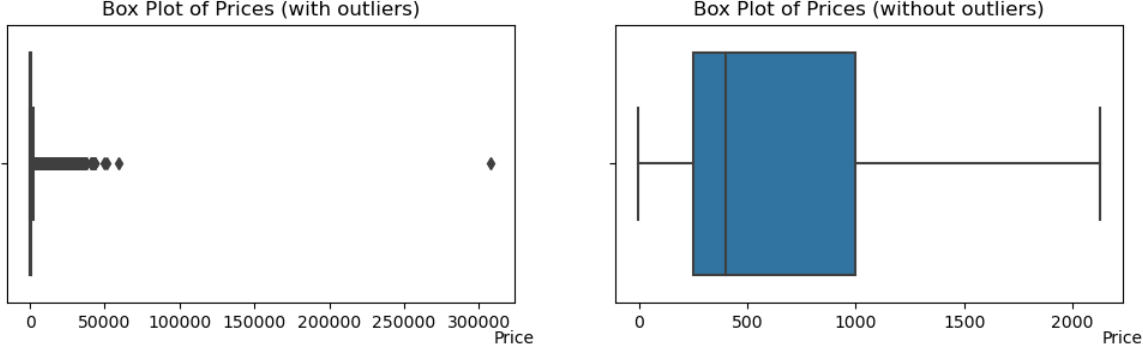
\includegraphics[width=14cm, height=3.8cm]{./figs/price-box.png}
    \caption{Box Plots of Prices}
    \label{fig:price-box}
\end{figure}

The third row in Table \ref{tab:de-stat} reveals some facts about the total sales by category. The large standard deviation indicates that the sales of items varies greatly from category to category. And the distribution is significantly right-skewed. The least-sold category has only one sale, while category 40 could even reach 600,000.


\subsection{Trends}
The changing trends in time-series data provide important insights for developing forecast models. We firstly study the relation between sales and month. Figure \ref{fig:month-sales} is a bar plot of the month and the total monthly sales.

\begin{figure}[!ht]
    \centering
    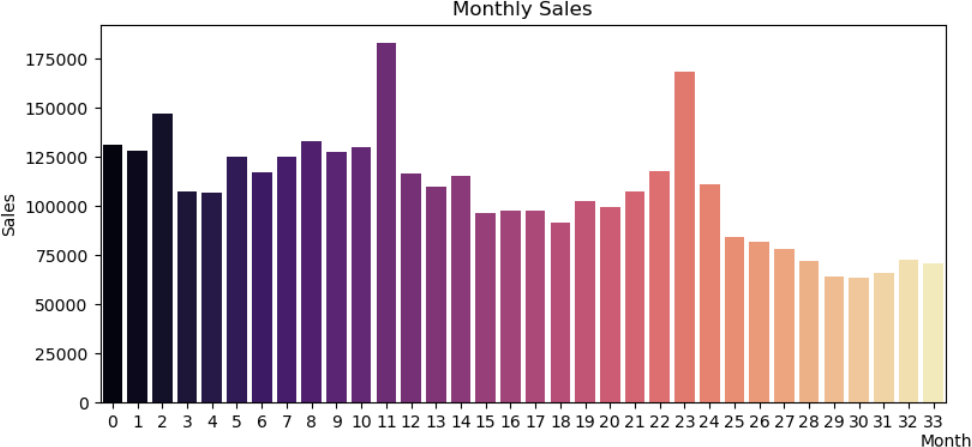
\includegraphics[width=12cm, height=4.5cm]{./figs/month-sales.png}
    \caption{Monthly Sales of Products}
    \label{fig:month-sales}
\end{figure}

From Figure \ref{fig:month-sales}, we can see that the sales in month 11, 23 (both November) are higher than others, which is probably due to Black Friday in November. This nearly 3-year period also witnessed a steady decline of sales year by year. Especially in the third year (from month 25), the sales is remarkably lower than previous.\par

The changing trend of each shop's daily sales is worth some exploration, too. We select 3 different shops: shop 25, shop 35, and shop 55. Figure \ref{fig:shop-sales} illustrates the changing trend of dailu sales. We can see that the sales around new year are the highest in a year for shop 25 and 35. But some shops may follow a different pattern. For example, shop 55 opened in May 2013. Its sales remained fairly low until a surge occurred in October 2014. The highest point of its sales is every October instead of January. But these shops all show a typical trend of sales in a yearly cycle.

\begin{figure}[!ht]
    \centering
    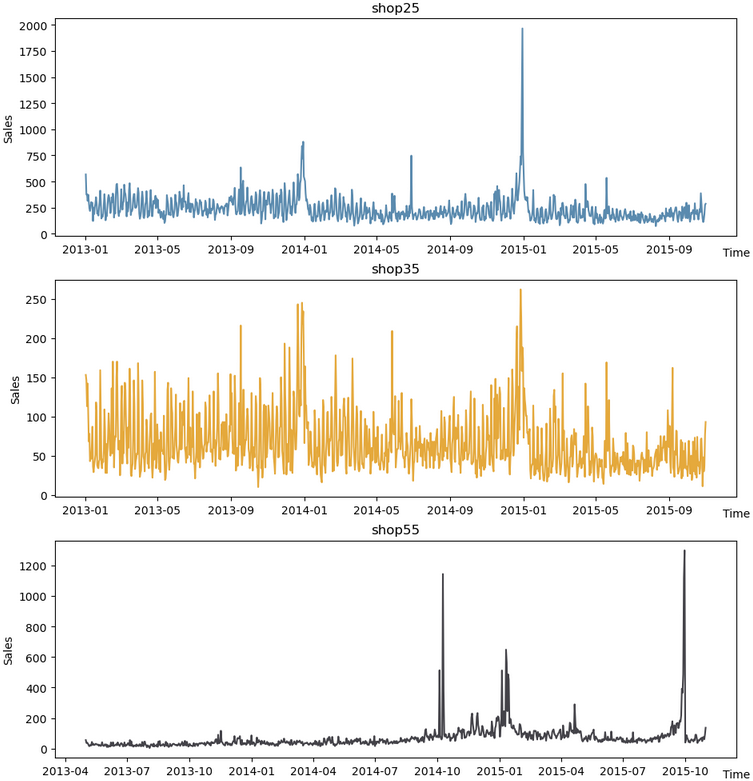
\includegraphics[width=12cm, height=9.35cm]{./figs/shop-sales.png}
    \caption{Daily Sales of Products}
    \label{fig:shop-sales}
\end{figure}

There is also one indicator we should follow: city. We focus on numbers of shops and average monthly sales in different cities. Figure \ref{fig:city} shows the number of shops in cities and average monthly sales of cities. It can be seen that Moscow has the most shops and highest average monthly sales. Many of other cities have only one or two shops and significantly lower sales than Moscow.

\begin{figure}[!ht]
    \centering
    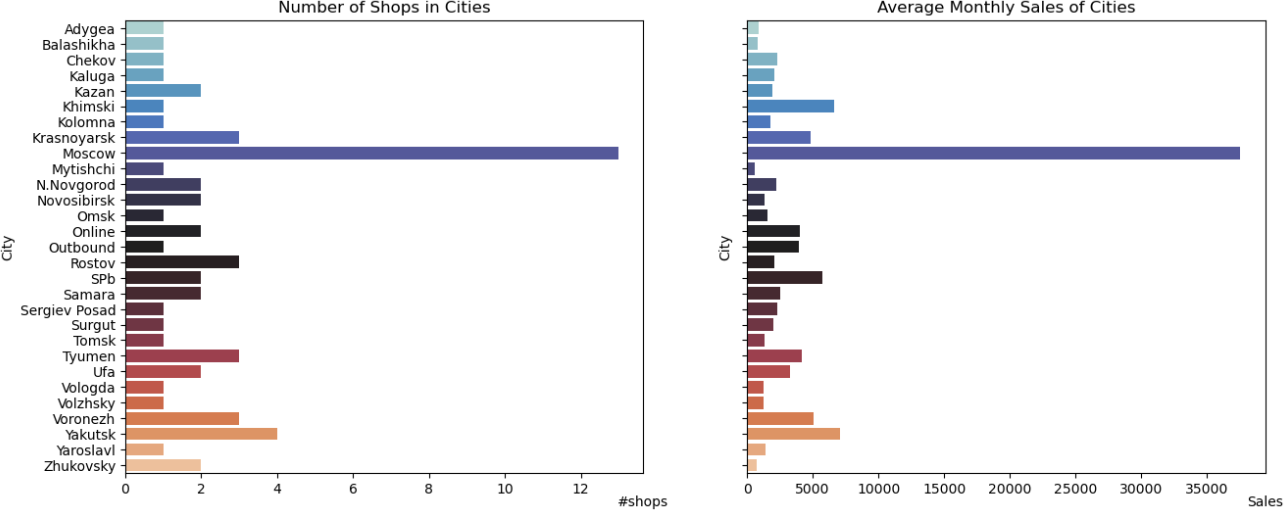
\includegraphics[width=16.5cm]{./figs/city-sales.png}
    \caption{Number of Shops in Cities and Average Monthly Sales of Cities}
    \label{fig:city}
\end{figure}

\section{Preprocessing and Feature Engineering}
We preprocess the data to remove anomalies found in exploratory data analysis. Besides, we also aggregate training data by month and add item records with zero monthly sales. Then, we extract features from the cleaned data for modeling stage. We consider both text embeddings and structural embeddings, which will be explained in detail in this section.

\subsection{Preprocessing}
According to descriptive statistics in Section \ref{stat}, there are two types of outliers in item prices -- the overly high price and the negative price. We substitude the negative price with the mean value of other records that have the same item id and date. We use the median of item prices later in feature engineering to diminish the impact of overly high prices and thereby don't deal with these records at the current stage.\par
Another obvious abnormality is the negative daily sales in training data. The number of records with negative daily sales reaches 7,356, which is unlikely caused by input errors. Our assumption is that the negative daily sales represents the number of refunded items. We replace these negative values by zero, for the sales of refunded items has already been taken into account in the previous records.\par
After handling anomalies, we aggregate the daily sales column to monthly sales, aiming at discovering the long-term trend and staying consistent with the test set. This operation reduces the number of records in the training set from 2,935,849 to 1,609,124.\par
It is also worth noting that the test set is the Cartesian product of all items and shops, while the training set only includes records whose sales is positive. The lack of zero sales records in training set increases the deviation between training data distribution and test data distribution. Therefore, we generate the Cartesian product of all items and shops and compute difference sets in the training data month by month. We extend the training data with these difference sets and assign zero to the sales. The number of records in the training set remarkably increases to 10,913,850. And this operation fixes the gap between two distributions. \par
Inspired by discussions on Kaggle forum, we notice that names of some shops are very similar. We guess the similarity is due to input errors or re-opening of the shop. Our scheme is merging the records of three pairs of shops with similar names, i.e., shop 0 and 57, shop 1 and 58, shop 10 and 11.

\subsection{Feature Engineering}
\subsubsection{Text Embeddings}
Textual contents include extensive information about the dataset. For the project, item name, shop name, and category name columns provide concise descriptions of relevant objects in Russian. We develop two tactics to fully utilize the text data. One is text mining, the other is pattern recognition.\par
We use pre-trained word2vec, tf-idf, and language translation to distill information from text. To obtain word vectors, we start with tokenizing the text data and then search for the corresponding pre-trained vectors in a Russian language model downloaded from \url{https://fasttext.cc/docs/en/pretrained-vectors.html}. Since the item name is usually a mixture of English and Russian, we only apply the word2vec model on shop name and category name. After that, we concatenate the vectors and pad them to the same length. The output of each record is a high-dimensional sparse vector and is not suitable for using directly as features. We convert the word vectors into some high-level features via the agglomerative clustering method. Figure \ref{fig:agg} shows the result of agglomerative clustering on the word vectors of item category name. 

\begin{figure}[!ht]
    \centering
    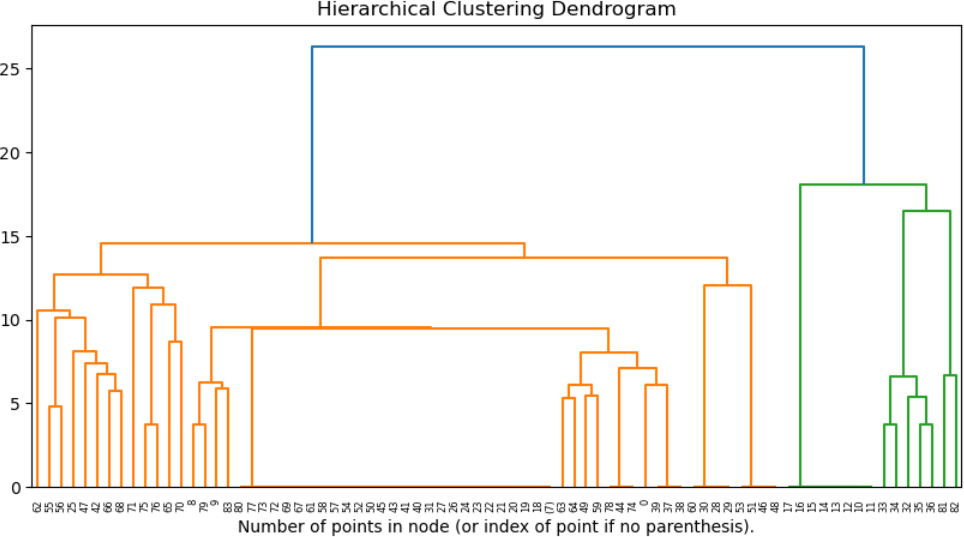
\includegraphics[width=10cm]{./figs/agg.png}
    \caption{Category Name: Clustering of Word Vectors}
    \label{fig:agg}
\end{figure}

As for item name, except for the multi-lingual problem mentioned before, the large volumn of item names is also a challenge for feature extraction. We tackle these challenges by calculating the tf-idfs of top-25 words in item names based on term frequency. Because none of us understand Russian, we also try to translate the text into English and manually create three features for shops and two hierarchical category features.\par
We also observe that there are some patterns in shop names and item names. The first Russian word in shop name is the city that the shop is located in. The next word usually indicates the type of the shop, followed by the name of the shop in quotation marks. Information about city and shop type is extracted from the original text and encoded as ordinal variables. Patterns in item name are harder to be detected. We use regular expressions to extract strings from parentheses in item names and select the strings appeared more than five times. We find that the text in parentheses are associated with the game platform, such as PC, Xbox, etc. The first word in item name also includes some important information about the item. For example, it may be the first word of the video game manufacturer or the game series. We treat the above patterns in item name as ordinal vatiables.

\subsubsection{Structural Embeddings}
We mainly extract four kinds of structural embeddings in the project.
\begin{itemize}
    \item[] \textbf{Date}. The date itself contains the information of year, quarter, and month. Given a specific month, we can easily create features like the number of days, the number of weekdays, etc. We also consider that holidays may affect the sales and compute the number of holidays in a month according to Russian holiday calendar.
   \item[] \textbf{Price}. As we all konw, sales of the product is related to the price of the product. We calculate the median of prices for each item month by month and fill the NaN values with zero.
   \item[] \textbf{Release Date}. There are several newly released products each month. It is reasonable to assume that the sales of the new product is better than that of the product existed for years, especially in software industry. Therefore, we create the release date feature for each item.
   \item[] \textbf{Lag}. In time series data, variables are highly time-correlated. Features reflected time correlation are helpful to improve model performance. We create lag features for monthly sales and price median of the first six months as well as twelve months. NaN values are filled with zero.
\end{itemize}

\section{Algorithms}
This section introduces the best three algorithms we have adopted in the Kaggle competition. Besides, we also explain our evaluation procedure and report the model performance. RMSE is selected as our metrics, which is consistent with Kaggle. 

\subsection{ARIMA}
The ARIMA model is a traditional statistical method designed for time series data. It combines autoregression and moving average techniques to forecast future trends based on historical observations. Therefore, its input is the previous sales data in this task and doesn't require manually selected features. Compared to sophisticated machine learning models, the ARIMA model is usually more robust and easier to use. We set the ARIMA model as baseline. Since the train set includes nearly two years' daily sales data, we incorporate seasonal terms in ARIMA model. Denoting the time span as $S$, our model can be written in the form of,
\begin{align*}
    ARIMA\left( p, d, q \right) \times\left( P, D, Q \right) S
\end{align*}
where $p$, $d$, $q$ are AR order, difference order, and MA order respectively. And the capital letters correspond to seasonal orders. The target of competition is predicting the monthly sales for each shop-item pair. However, if we create ARIMA models for each shop-item pair, there will be a major difficulty. Although the volume of training data is large, samples amortized for each pair are insufficient to provide enough information about trending to train the ARIMA model. To ensure the validity of ARIMA, we model the monthly sales for each shop and estimate the sales of each item by multiplying the shop sales prediction and the share of the item sales out of total sales. We take shop 2 as an example. Figure \ref{fig:arima-1} is the result of model diagnostics, which supports the model validity. And Figure \ref{fig:arima-2} depicts the original monthly sales data as well as the prediction. According to Figure \ref{fig:arima-2}, the prediction of ARIMA model is reasonable.\par

\begin{figure}[!ht]
    \centering
    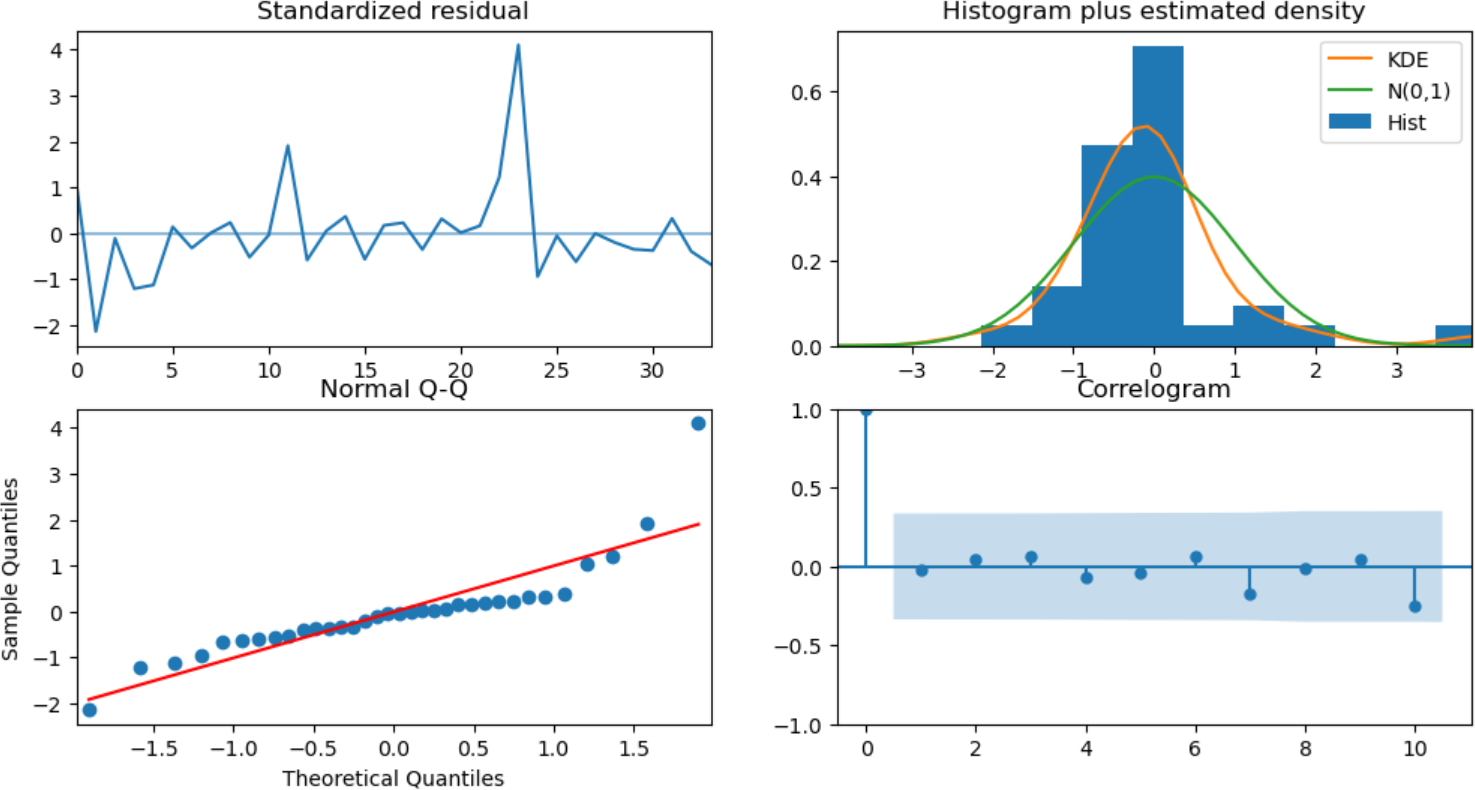
\includegraphics[width=10cm]{./figs/arima-1.png}
    \caption{Shop 2: ARIMA Model Diagnostics}
    \label{fig:arima-1}
\end{figure}

\begin{figure}[!ht]
    \centering
    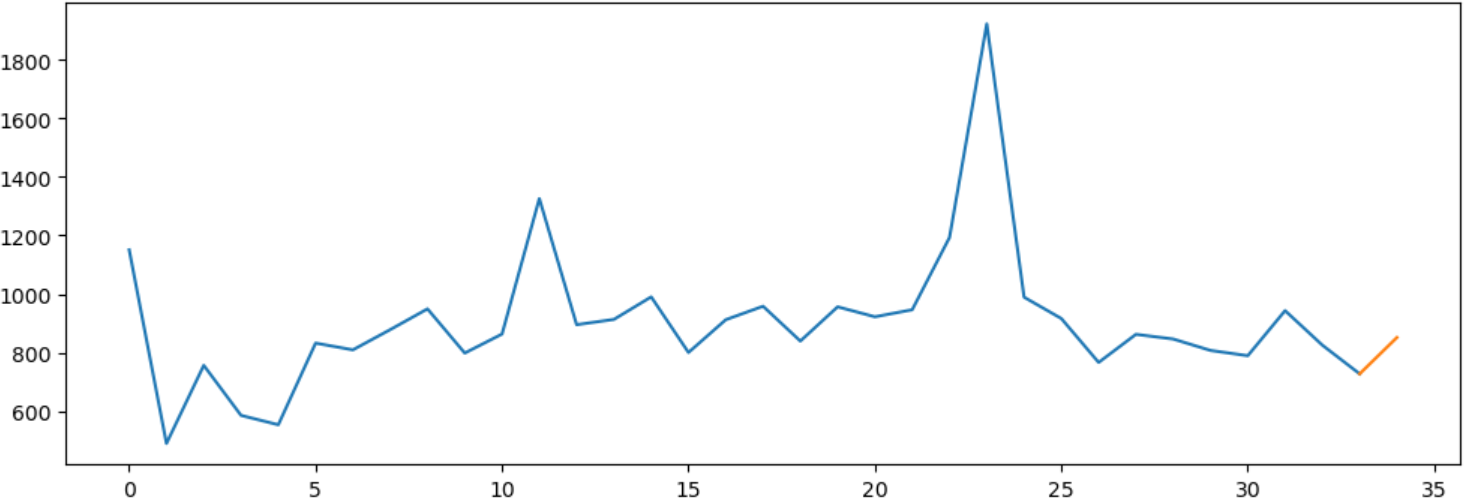
\includegraphics[width=10cm]{./figs/arima-2.png}
    \caption{Shop 2: ARIMA Model Prediction}
    \label{fig:arima-2}
\end{figure}

The standard procedure of creating the ARIMA model is manually setting the parameters related to orders based on model diagnostics. However, it will be laborious if we repeat the parameter selection for all shops. We automate the procedure by using \texttt{auto\_arima} API in pmdarima package. After obtaining shops' monthly sales predictions, we generate the prediction for each shop-item pair with the strategy mentioned before. Items released in November 2015 don't have historical sales data and lead to NaN values. We fill these NaN values with the average value of predictions. RMSE of ARIMA model on test set is 1.18663.

\subsection{Blending Model} \label{method}
Stacking and blending are two commonly used strategies in Kaggle competitions. Model stacking requires cross validation during the training, which may cause information leakage in time series data. Thus, we choose model blending method in our project. Figure \ref{fig:blending} illustrates the model architecture that we design for the dataset.

\begin{figure}[!ht]
    \centering
    
\includegraphics[width=16cm]{./figs/blending.png}
    \caption{Blending: Model Architecture}
    \label{fig:blending}
\end{figure}

Considering the time series nature of the dataset, we select the sales data in October 2015 as validation set and use the data before October 2015 as training set. Firstly, we train two base learners, CatBoost and XGBoost, on training set to obtain predictions on validation set and test set. After that, we regard predictions as new features and merge them into validation set and test set. These augmented data sets are the inputs of the meta model, which is Histogram-based gradient boosting regression tree in our blending model. Specifically, the meta model is fitted on the augmented validation set and output final predictions based on the augmented test set. Table \ref{tab:blending} summarizes the key parameter settings in the blending model. \par

\begin{table}[!ht]
    \centering
    \caption{Blending: Parameter Settings}
    \label{tab:blending}
    \begin{tabular}{lll}
        \toprule
        \textbf{Parameter} & \textbf{Value} & \textbf{Meaning}\\
        \midrule
        early\_stopping\_rounds & 10 & The number of early stopping rounds in CatBoost and XGBoost.\\
        n\_estimators & 5000 & The number of estimators in XGBoost.\\
        max\_depth & 10 & Maximum depth of a tree in XGBoost.\\
        learning\_rate & 0.1 & Learning rate in XGBoost.\\
        subsample & 0.5 & Subsample ratio of the training instances in XGBoost.\\
        \bottomrule
    \end{tabular}
\end{table}

The performance of blending model is better than ARIMA model, whose RMSE on test set is 0.98551.

\subsection{XGBoost}
During the training of blending model, we find that the performance of XGBoost on validation set is better than that of CatBoost. We conjecture using XGBoost alone may produce more accurate predictions. We split the traing data into training set and validation set in the same way as Section \ref{method}. Besides, we use the same parameter settings in Table \ref{tab:blending} for XGBoost. According to results of Kaggle submissions, XGBoost outperforms other two models with 0.93308 RMSE.\par

We perform a feature importance analysis to provide some insights into the effectiveness of XGBoost. F scores of all features can be found in the jupyter notebook. According to the feature importance plot, the median of item's monthly prices and lag values of item's historical sales contribute most to XGBoost's performance.

\subsection{Evaluation Procedure}
Before submission, we clip predictions into the valid range $[0, 20]$. The strategy of generating predictions from the ARIMA model creates a barrier to assess RMSE before submission. As for blending model, we can only infer the model performance from base learners, because the input of the meta model is an augmented version of the validation set. The average of base learners' RMSE is 0.89203. The evaluation of XGBoost model is straightforward, i.e., we can directly calculate RMSE on the validation set. RMSE of XGBoost on validation set is 0.88883. Table \ref{tab:evaluation} summarizes our evaluation results before submission and the real RMSE computed by Kaggle.

\begin{table}[!ht]
    \centering
    \caption{Summary of Evaluation}
    \label{tab:evaluation}
    \begin{tabular}{lll}
        \toprule
        \textbf{Model} & \textbf{Validation RMSE} & \textbf{Test RMSE}\\
        \midrule
        ARIMA & - & 1.18663\\
        Blending Model & 0.89203 & 0.98551\\
        XGBoost & \textbf{0.88883} & \textbf{0.93308}\\
        \bottomrule
    \end{tabular}
\end{table}

\section{Conclusion}
Kaggle competitions with regards to tabular data follow a three-stage workflow: exploratory data analysis, preprocessing and feature engineering, modeling. Exploratory data analysis provides some basic information about data, for example, the existence of missing values or outliers. Plots and descriptive statistics are helpful to avoid disastrous mistakes later in feature engineering and modeling. Preprocessing and feature engineering are higly data-driven. Some information are contained in the text descriptions, e.g. the city appears as the first word in the shop name. Some information are given implicitly and hard to be realized. For instance, the item with zero sales would not be recorded in the training set, which may lead to the bias in model. There are various algorithms for time series data, from the traditional ARIMA to the state-of-the-art XGBoost. The performance of model depends on the quality of features and properties of data. We go through the three-stage process in the project and finally rank in top 35\% on the Kaggle competition.

\end{document}
